\documentclass[hyperref=colorlinks]{beamer}
\mode<presentation>
\usetheme{iclpt}
\setbeamertemplate{navigation symbols}{}
\setbeamertemplate{headline}{
  \begin{beamercolorbox}[leftskip=.2cm,rightskip=.2cm,topskip=.2cm,ht=1.1cm,dp=0.1cm,wd=\textwidth]{institute in head/foot}
    
\includegraphics[height=1cm]{icl.pdf}
    \hfill
%    \includegraphics[height=1cm]{../Pics/ATLAS-Logo-Square-Blue-RGB.png}
%    
\includegraphics[height=1cm]{../Pics/CMS-Color.pdf}
    
\includegraphics[height=1cm]{TalkPics/t2k_logo_large.png}

%??put t2k logo here
  \end{beamercolorbox}
}
\setbeamertemplate{footline}{
  \begin{beamercolorbox}[ht=.35cm,dp=0.2cm,wd=\textwidth,leftskip=.3cm]{author in head/foot}%
    \begin{minipage}[c]{5cm}%
      \usebeamerfont{author in head/foot}
      \insertshortauthor 
      \insertshorttitle
    \end{minipage}\hfill%
    \hfill
    \insertframenumber{} / \ref{lastframe}
    %\hfill
    \begin{minipage}{6cm}
      \hfill
      %\insertshorttitle
    \end{minipage}
  \end{beamercolorbox}%
}

\definecolor{beamer@icdarkblue}{RGB}{0,51,102}
\definecolor{beamer@icmiddleblue}{RGB}{0,82,150} 
\definecolor{beamer@iclightblue}{RGB}{200,212,232}
\definecolor{beamer@icmiddlered}{RGB}{204,51,0}
\definecolor{beamer@iclightred}{RGB}{232,212,32}

\usepackage{tikz}
\usetikzlibrary{arrows,shapes,backgrounds}
\usepackage{color}
\usepackage{tabularx,colortbl}
\usepackage{graphicx}
\usepackage{pdfpages}
\usepackage{feynmp}
\usepackage{rotating}
\usepackage{moresize}
\usepackage{slashed}
\usepackage{xcolor,colortbl}
\DeclareGraphicsRule{*}{mps}{*}{}
\hypersetup{colorlinks=false}

\title[Transverse Variables for HPTPC]{\vspace{-0.2cm} Model Sensitivity and Variables for HPTPC}
\author[P. Dunne]{Patrick Dunne - Imperial College London}
\titlegraphic{
  \vspace{-0.4cm}
}
\date{}
\begin{document}
\tikzstyle{every picture}+=[remember picture]
\tikzstyle{na} = [baseline=-.5ex]
\begin{fmffile}{t2ktemplatefeyndiags}


  %TITLE PAGE
  %20 mins + 5 questions
  \section{Title}
  \begin{frame}
    \titlepage
  \end{frame}

  \begin{frame}
    \frametitle{Overview}
    \begin{block}{}
        \scriptsize
        \begin{itemize}
        \item Will present a preliminary study on 2p2h model sensitivity of the HPTPC
        \item[-] Previous presentation on Single Transverse Variables (STV)
        \item Will show more information on hadron kinematics and new transverse variables
      \end{itemize}
    \end{block}
  \end{frame}

  \begin{frame}
    \frametitle{Single Transverse Variables - Reminder and Naming}
    \vspace{-.3cm}
    \begin{itemize}
    \item Use hadronic information to estimate nuclear effects
    \item Variables are all used frequently at hadron colliders
    \item[-] Naming that is emerging in neutrino physics is different
    \item[-] In hadron colliders: $\delta p_{T}=p_{T}^{miss}$, $\delta\phi_{T}=\pi-\Delta\phi(lep,had)$, $\delta\alpha_{T}=\pi-\Delta\phi(lep,p_{T}^{miss})$
    \item Personally find hadron collider naming more intuitive
    \end{itemize}
    \vspace{-.1cm}
    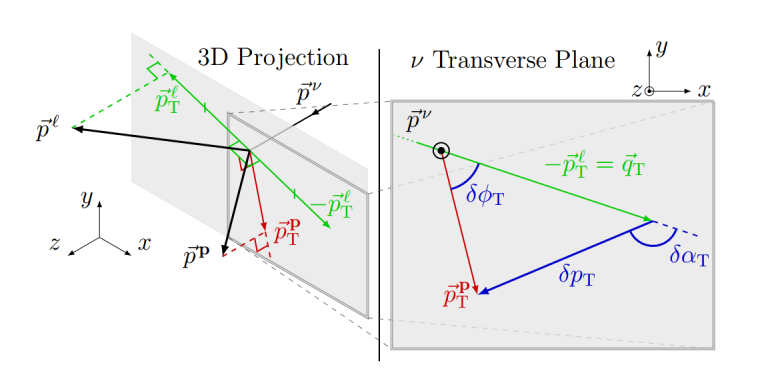
\includegraphics[width=\textwidth,clip=true,trim=0 0 0 20]{TalkPics/STVforHPTPC_101016/stvdiagram.png}
  \end{frame}

  \begin{frame}
    \frametitle{Other Transverse Variables - Reminder}
    \begin{itemize}
    \item Particularly for $p_{T}^{miss}$ context is important
    \end{itemize}
    \begin{block}{}
      \centering
      \begin{fmfgraph*}(60,50)
        \fmftop{i1,m1,m2,m3,m4,m5,m6,m7,o1}
        \fmfbottom{i2,m8,m9,m10,m11,o2}
        \fmf{fermion,tension=4}{v1,i2}
        \fmf{fermion,tension=4}{v1,o2}
        \fmf{fermion}{v1,m1}
        \fmf{dashes}{v1,m3}
        \fmf{fermion}{v1,m4}
        \fmf{fermion}{v1,m5}
        \fmf{fermion}{v1,m6}
        \fmf{fermion}{v1,m7}
        \fmf{fermion}{v1,m8}
        \fmf{fermion}{v1,m9}
        \fmf{fermion}{v1,m10}
        \fmf{fermion}{v1,m11}
      \end{fmfgraph*}
      \hspace{1.5cm}
      VS
      \hspace{1.5cm}
      \begin{fmfgraph*}(60,50)
        \fmftop{i1,m1,m2,m3,m4,m5,m6,m7,o1}
        \fmfbottom{i2,m8,m9,m10,m11,o2}
        \fmf{fermion,tension=4}{v1,i2}
        \fmf{fermion,tension=4}{v1,o2}
        \fmf{fermion}{v1,m1}
        \fmf{dashes}{v1,m3}
      \end{fmfgraph*}
      \vspace{.2cm}
    \end{block}
    \begin{itemize}
    \item Both events have the same $p_{T}^{miss}\delta p_{T}$ but on the right this is clearly more significant compared to uncertainties on visible object momenta
    \end{itemize}
    
  \end{frame}


  \begin{frame}
    \frametitle{HPTPC Study - Reminder}
    \begin{itemize}
    \item HPTPC-like and ND280-like momentum thresholds (below) and efficiencies (see Mark's talk 10th October) were applied to ND280 MC truth
    \item[-] Same as shown previously
    \item Then calculated transverse variables
    \item[-] Only make sense in samples with a proton or a pion
    \end{itemize}
    \begin{tabular}{l|cc}
      \hline
      Particle & ND280 Threshold/MeV & HPTPC Threshold/MeV \\
      \hline
      $\mu$ & 100 & 15 \\
      $\pi$ & 120 & 16 \\
      $p$ & 450 & 60 \\
      $e$ & 100 & 1 \\
      \hline
    \end{tabular}
  \end{frame}

  \begin{frame}
    \frametitle{HPTPC Study}
    \begin{itemize}
    \item Truth information is used to determine which events truly belong in the sample (``correct''), and which are ``fakes''
    \item[-] Distributions of transverse variables are shown for both
    \item Have seen previously that transverse variables look similar in ND280 and HPTPC
    \item Will show today effect of 2p2h model on variable shapes in ND280 and HPTPC
    \item[-] 2p2h Describes interactions between neutrino and 2 nucleons
    \item[-] MC is generated with Nieves model
    \item[-] Use reweighting to study Martini model
    \end{itemize}
  \end{frame}

  %??some plots for HPTPC and ND280 showing not much difference
  \begin{frame}
    \frametitle{CC0$\pi$1p}
    \begin{itemize}
    \item Look at sample with 1 proton and no pions
    \item Compare detectors (N events is arbitrary)
    \end{itemize}
    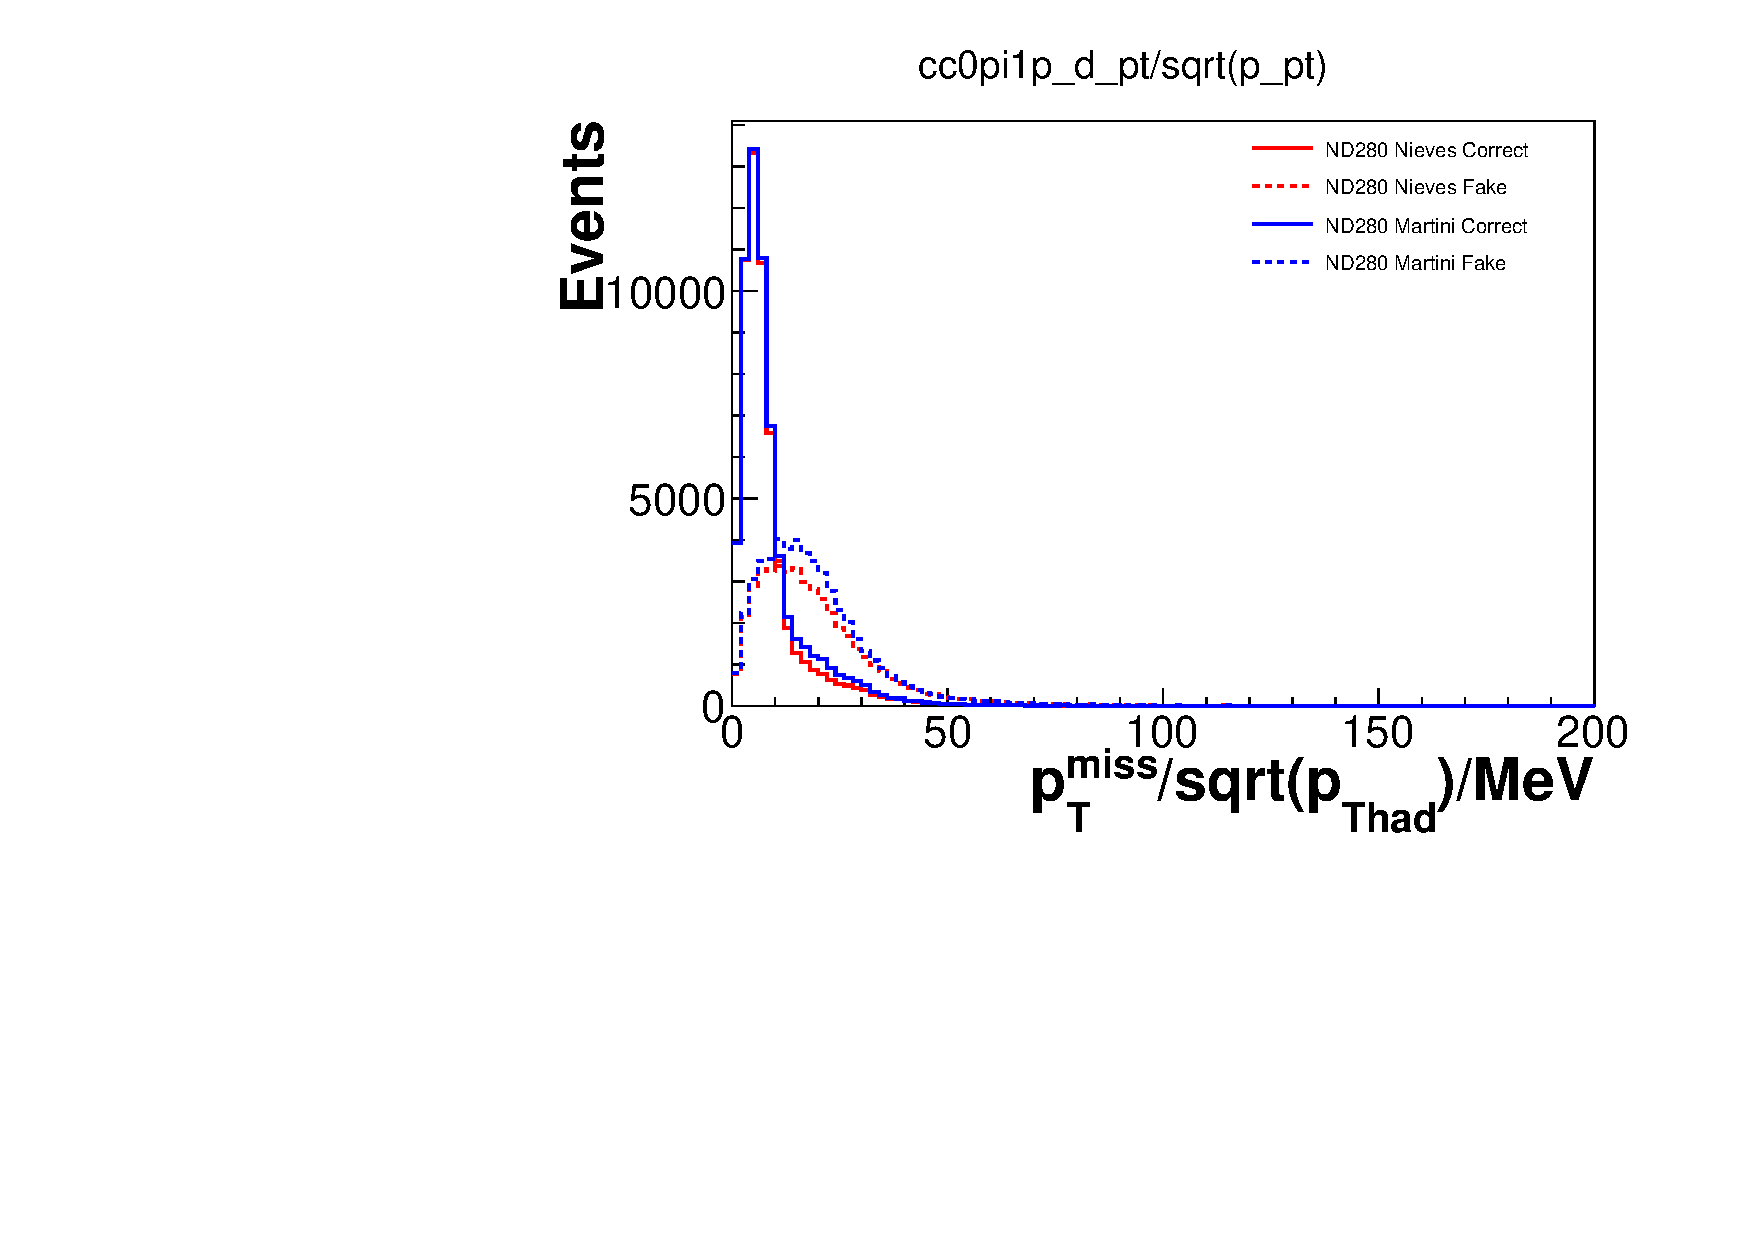
\includegraphics[width=.5\textwidth]{TalkPics/STVforHPTPC_191216/plots_martininievesnd280/cc0pi1p_metsig.pdf}
    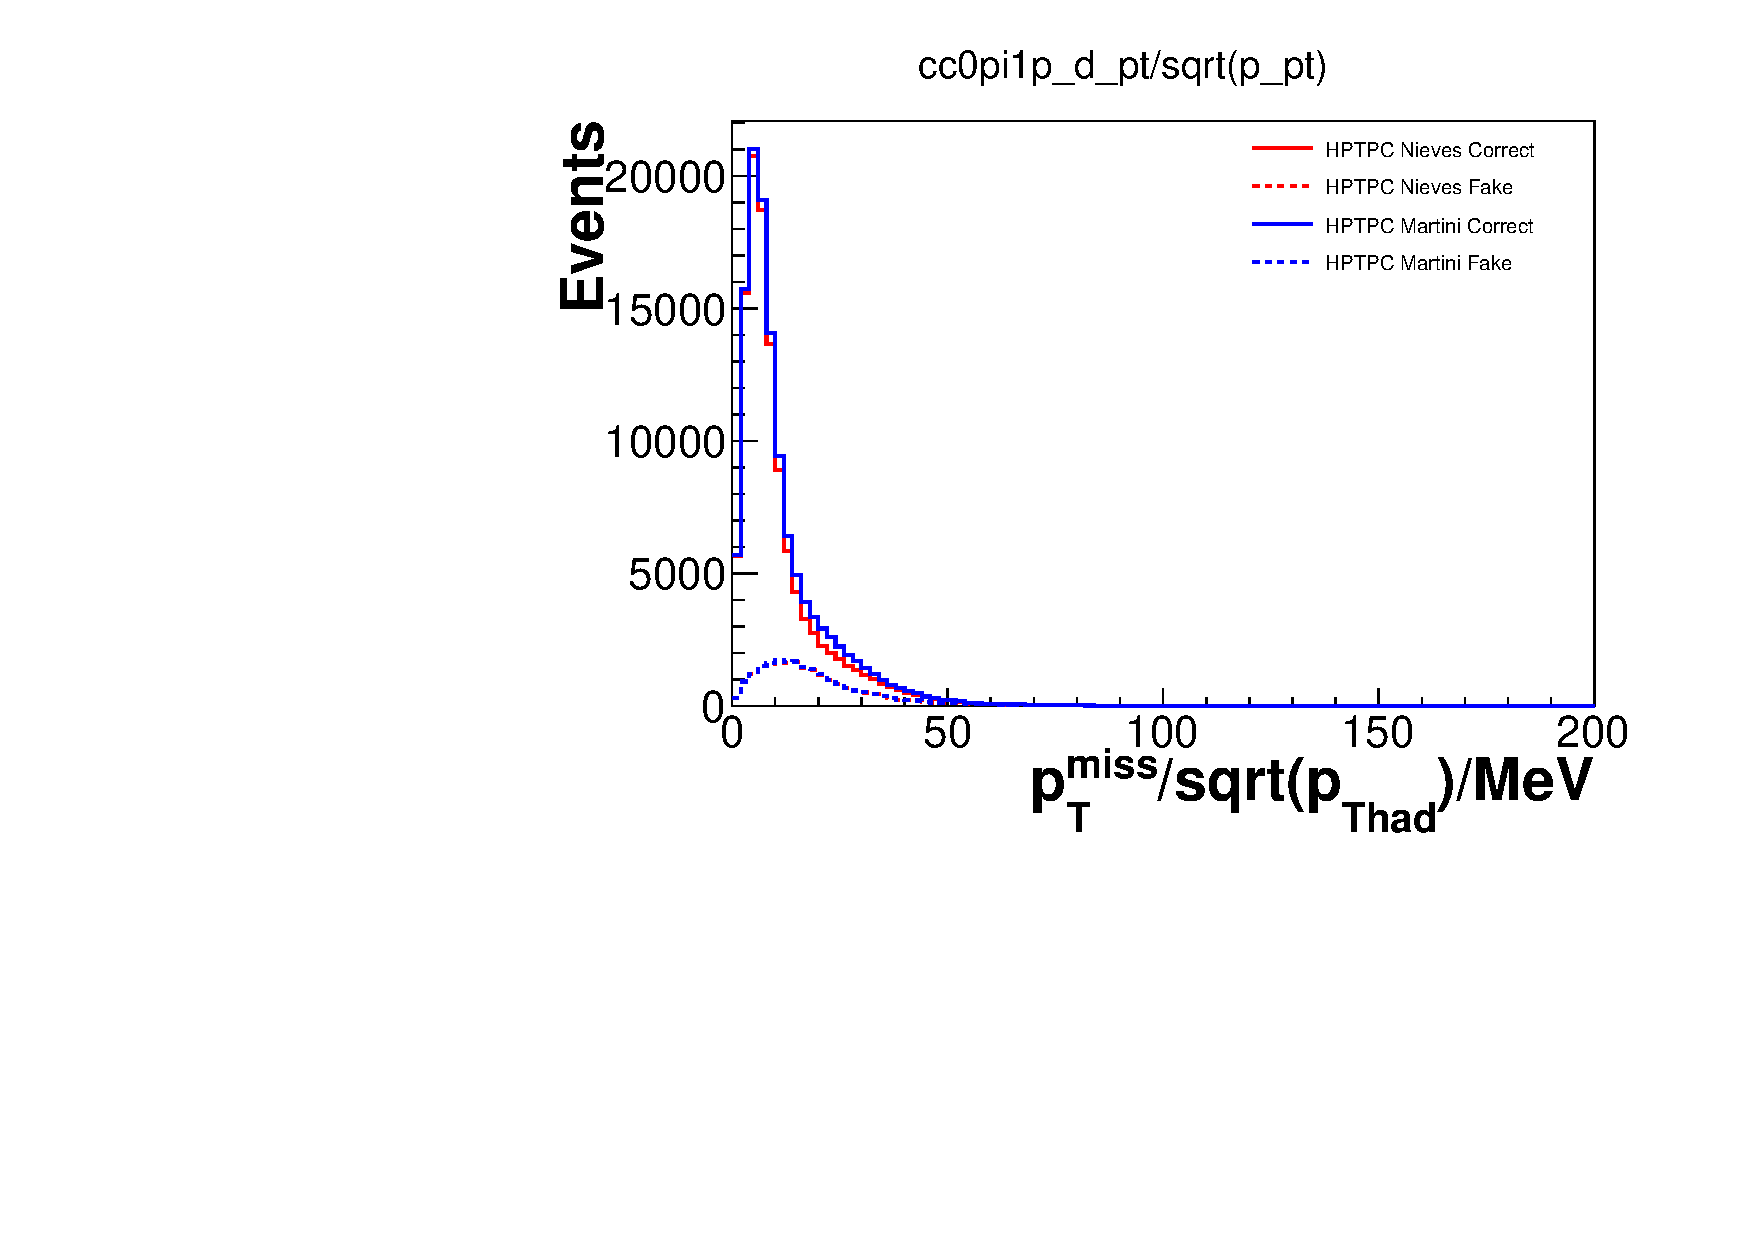
\includegraphics[width=.5\textwidth]{TalkPics/STVforHPTPC_191216/plots_martininieveshptpc/cc0pi1p_metsig.pdf}
  \end{frame}

  \begin{frame}
    \frametitle{CC0$\pi$1p}
    \begin{itemize}
    \item Look at sample with 1 proton and no pions
    \end{itemize}
    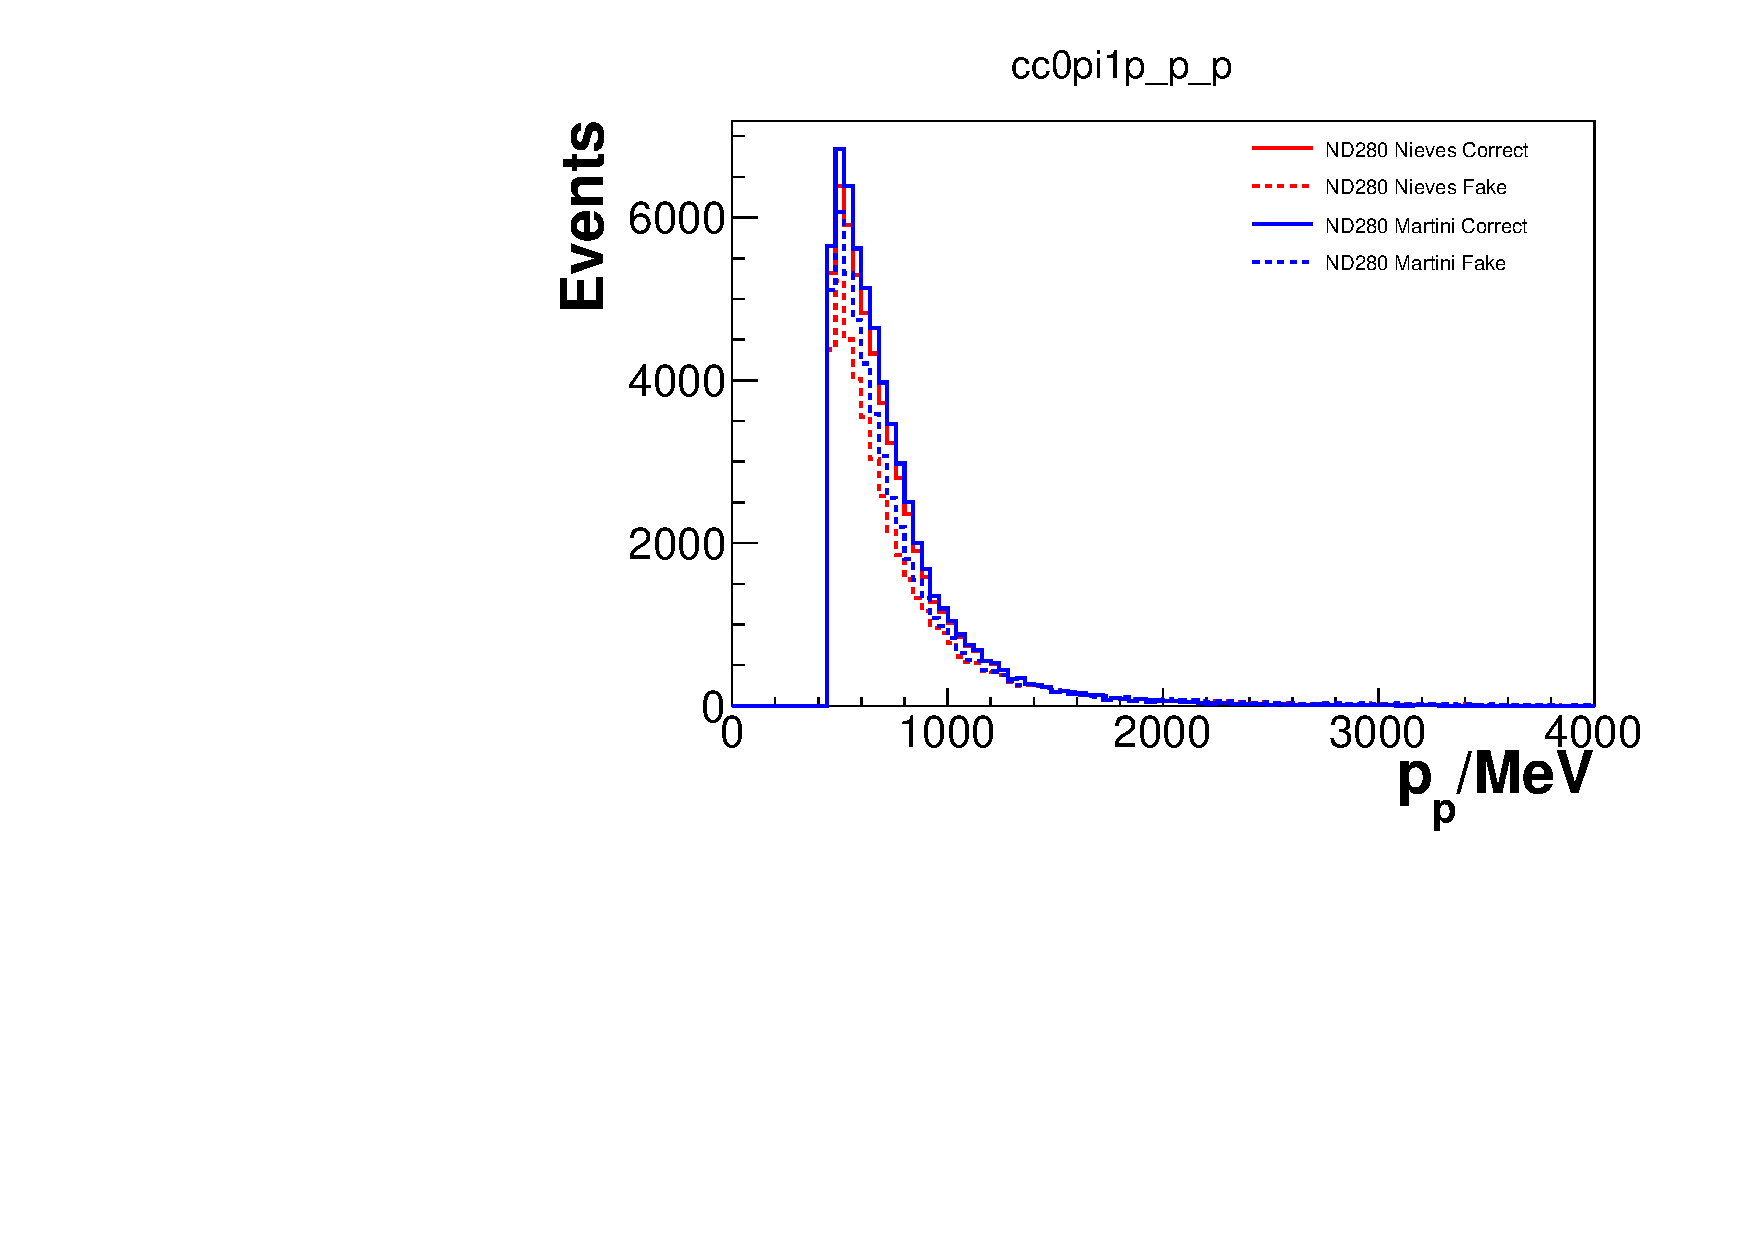
\includegraphics[width=.5\textwidth]{TalkPics/STVforHPTPC_191216/plots_martininievesnd280/cc0pi1p_p_p.pdf}
    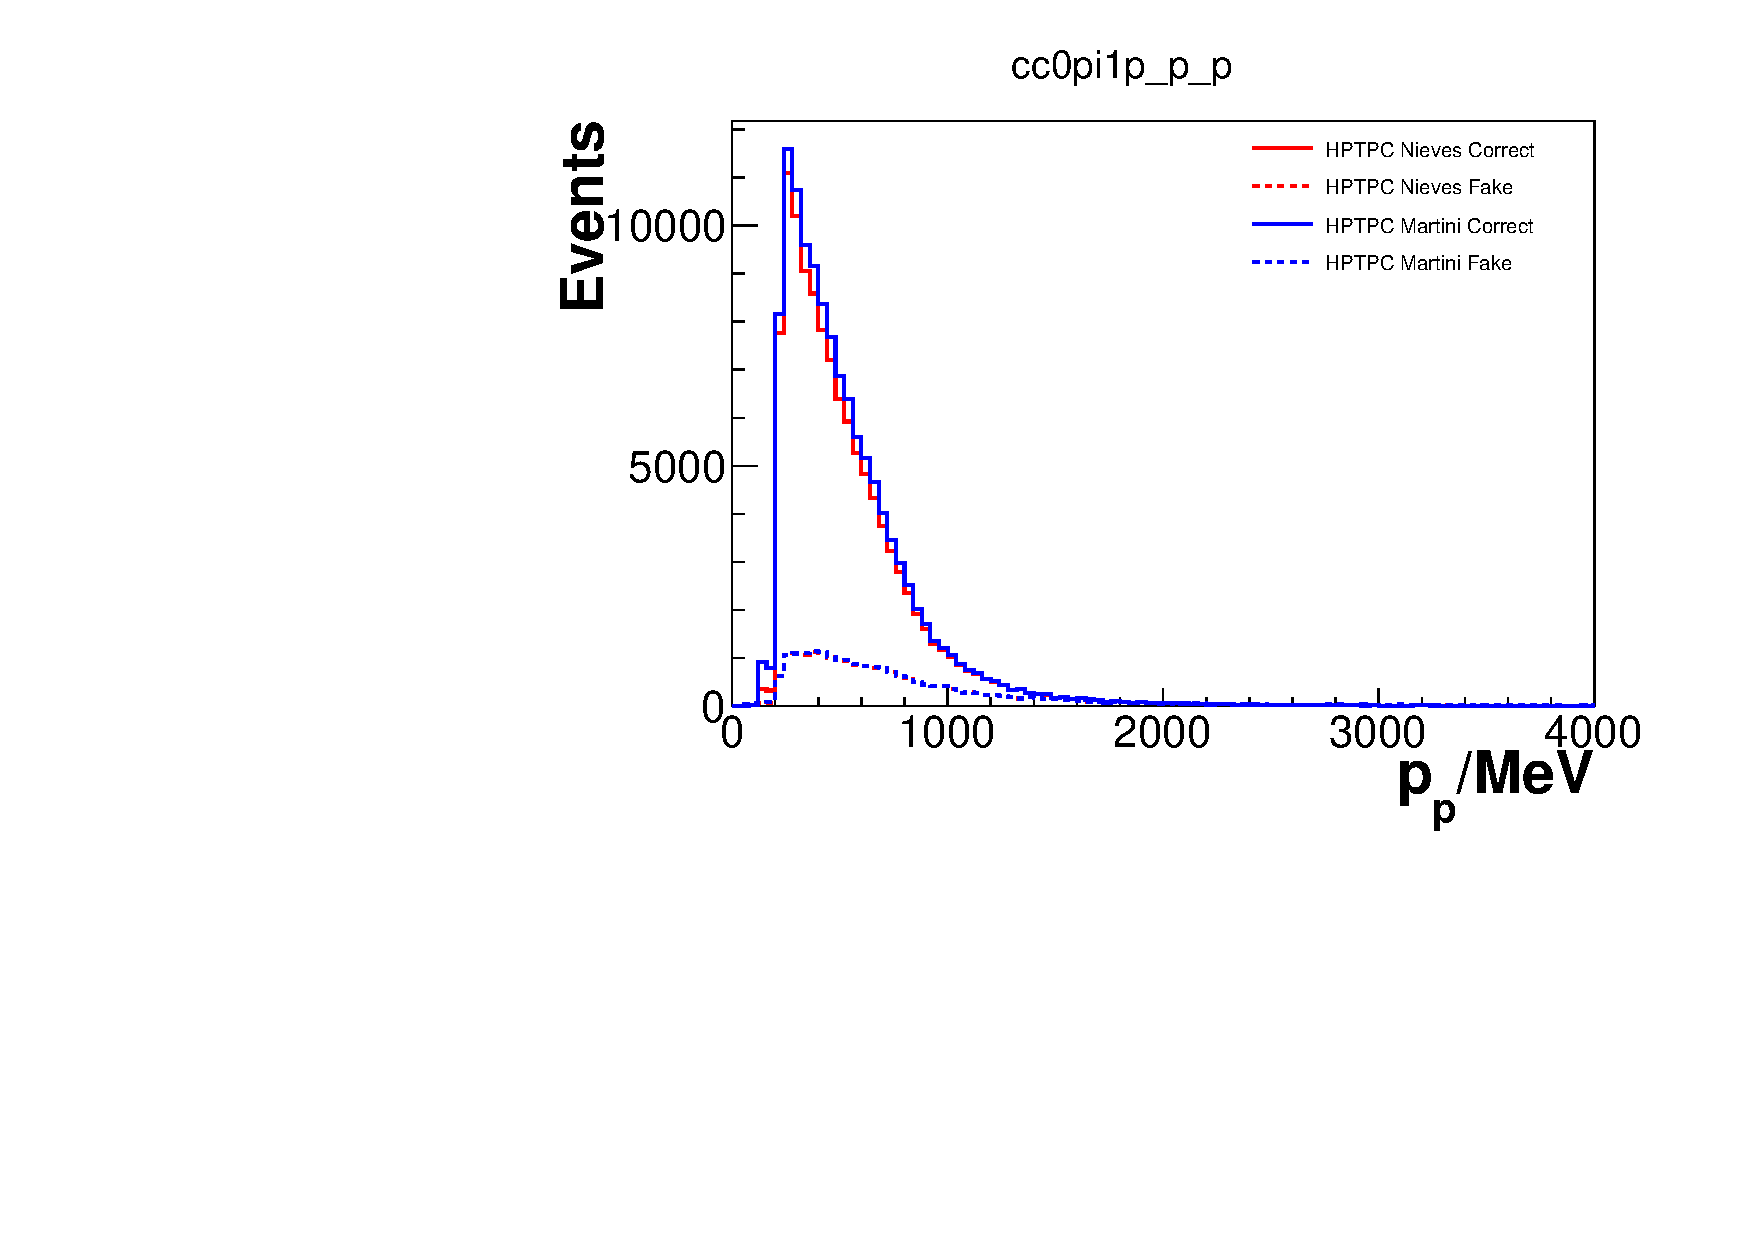
\includegraphics[width=.5\textwidth]{TalkPics/STVforHPTPC_191216/plots_martininieveshptpc/cc0pi1p_p_p.pdf}
  \end{frame}

  \begin{frame}
    \frametitle{Discussion of 2p2h}
    \begin{itemize}
    \item Results from CC0$\pi$1p don't show much discriminating power from HPTPC
    \item Expect there may be more power in CC0$\pi$Np because Martini and Nieves predict different proton multiplicities
    \item[-] Caveat, reweighting is only done as a function of $E_{\nu}$ so may not accurately describe hadron kinematics
    \end{itemize}
  \end{frame}
  
  \begin{frame}
    \frametitle{CC0$\pi$Np}
    \begin{itemize}
    \item Look at sample with $>=$1 proton and no pions
    \item Compare detectors (N events is arbitrary)
    \end{itemize}
    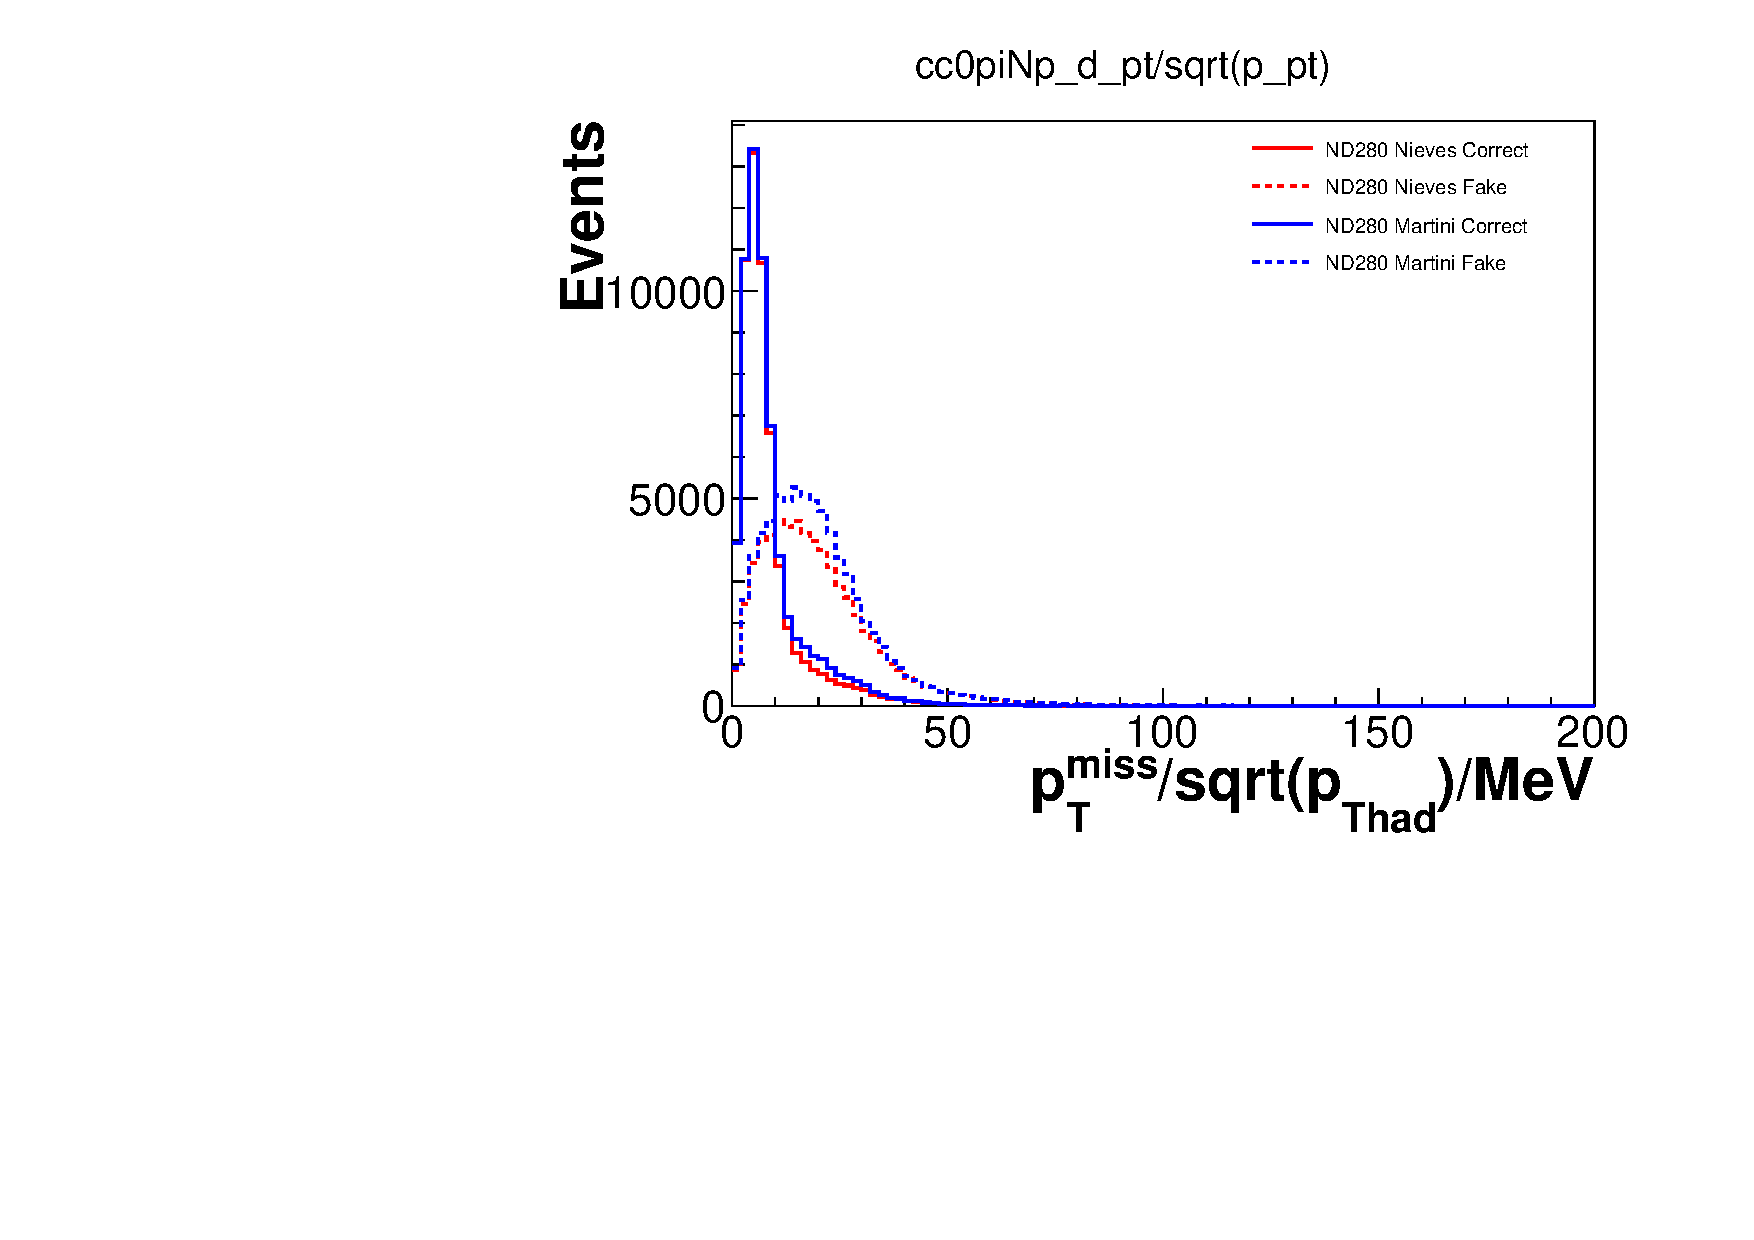
\includegraphics[width=.5\textwidth]{TalkPics/STVforHPTPC_191216/plots_martininievesnd280/cc0piNp_metsig.pdf}
    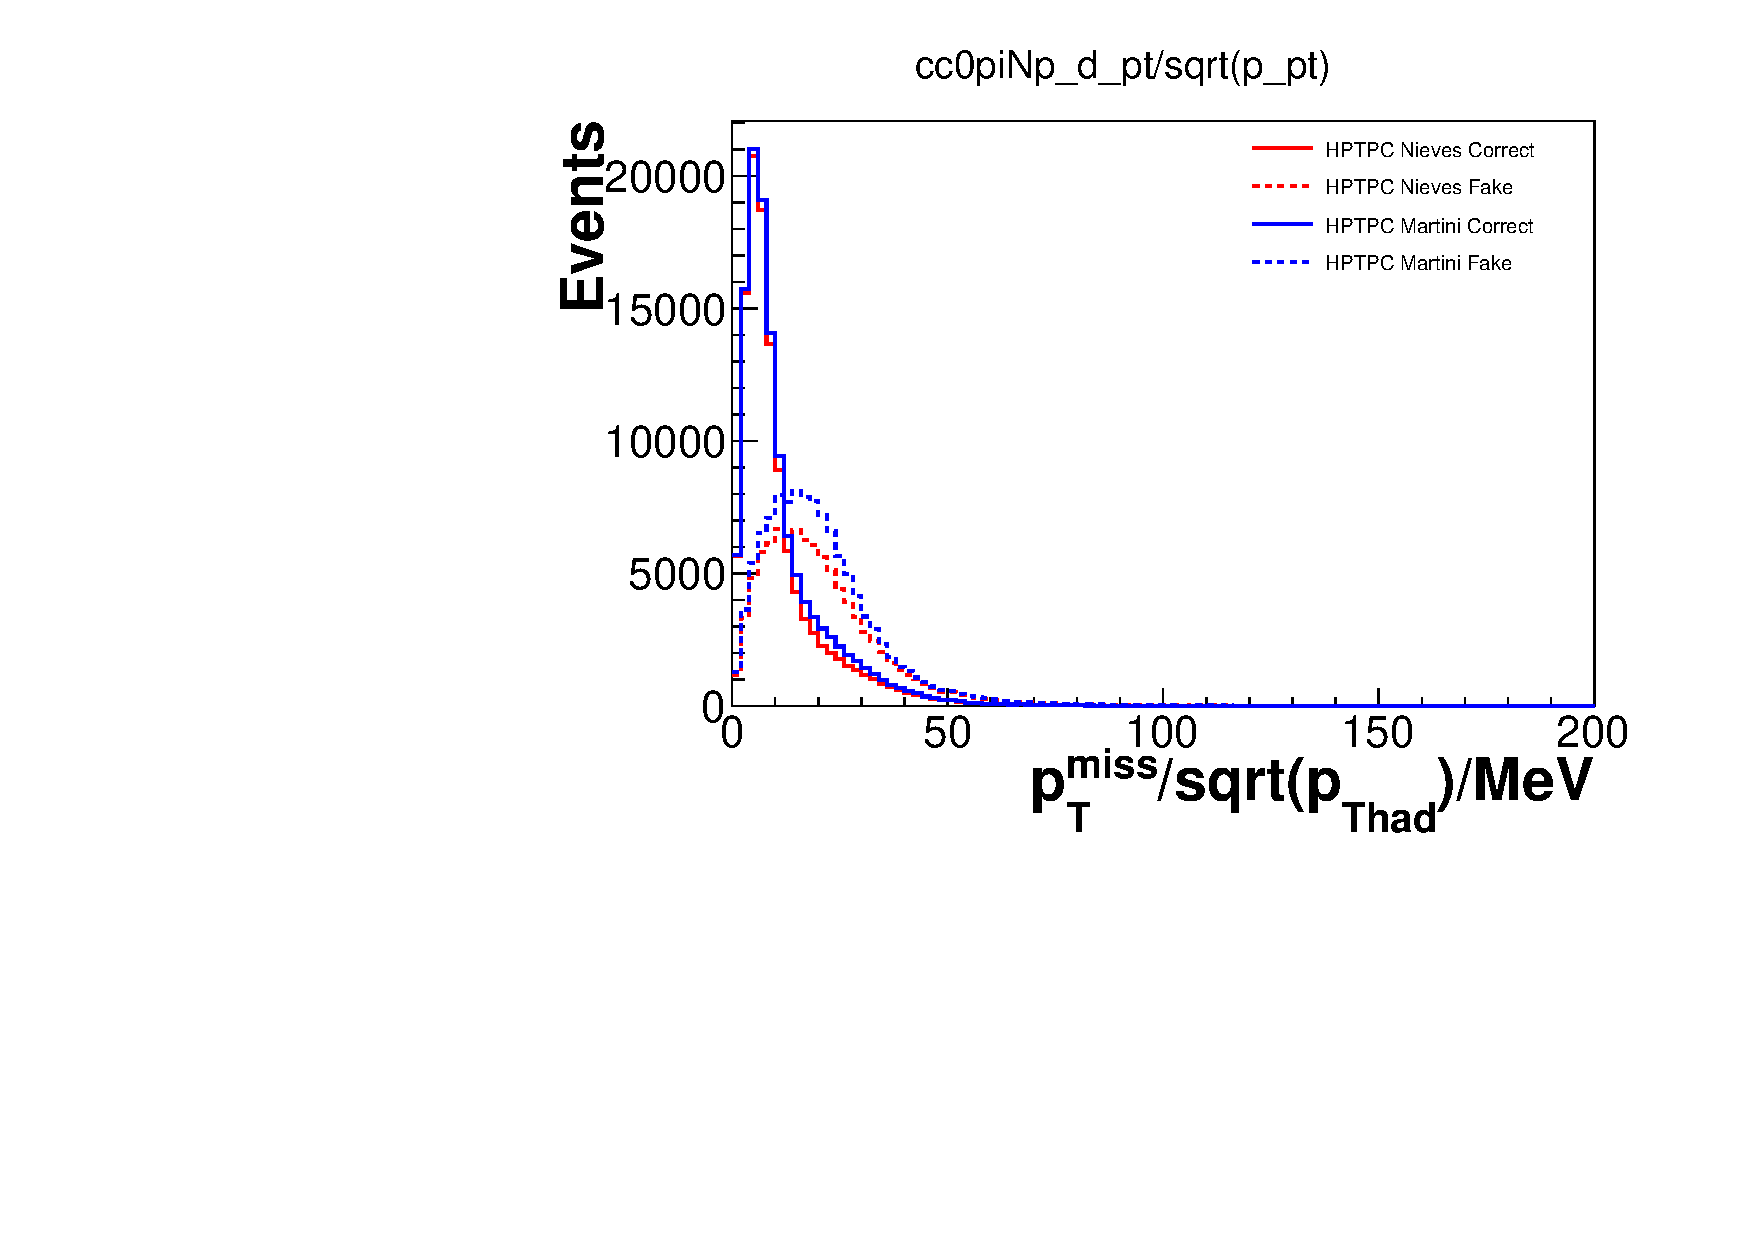
\includegraphics[width=.5\textwidth]{TalkPics/STVforHPTPC_191216/plots_martininieveshptpc/cc0piNp_metsig.pdf}
  \end{frame}

  \begin{frame}
    \frametitle{CC0$\pi$Np}
    \begin{itemize}
    \item Look at sample with $>=$1 proton and no pions
    \end{itemize}
    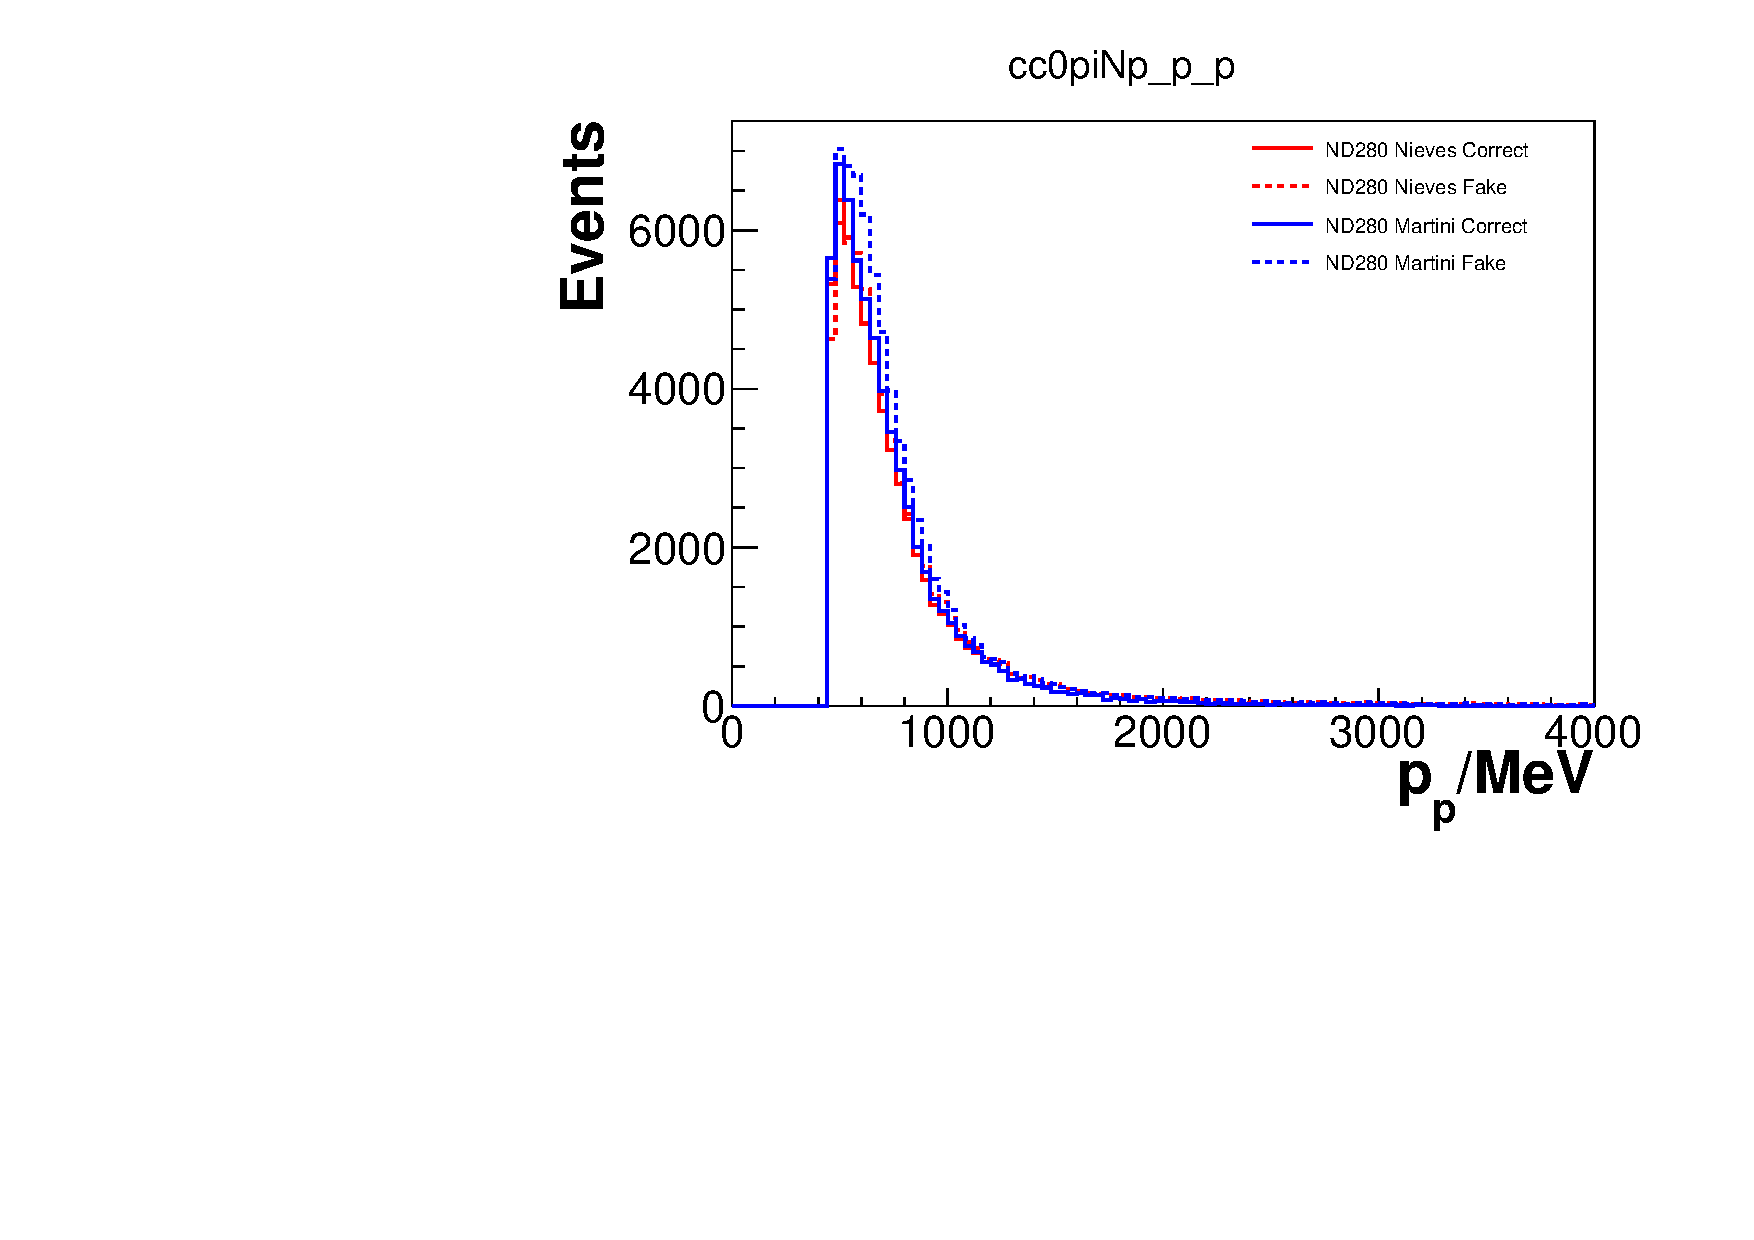
\includegraphics[width=.5\textwidth]{TalkPics/STVforHPTPC_191216/plots_martininievesnd280/cc0piNp_p_p.pdf}
    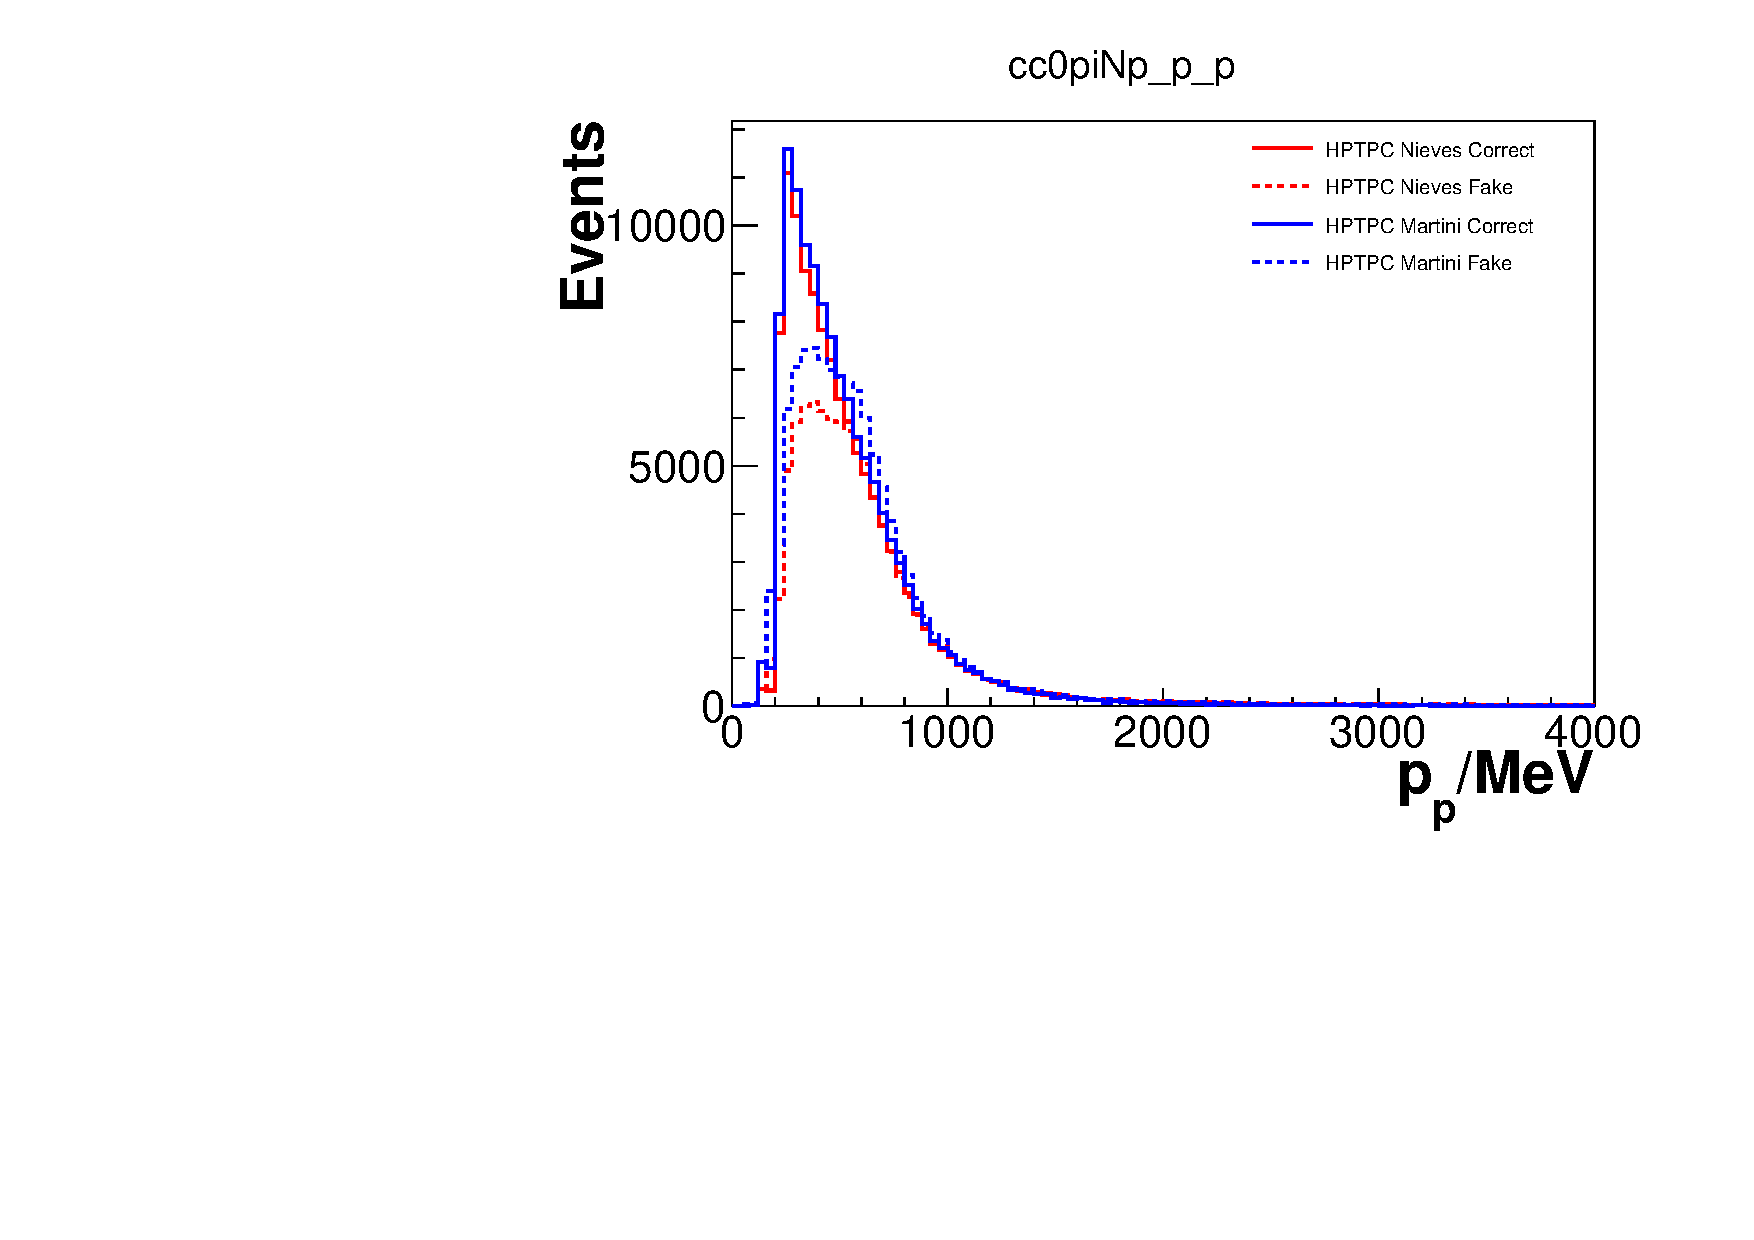
\includegraphics[width=.5\textwidth]{TalkPics/STVforHPTPC_191216/plots_martininieveshptpc/cc0piNp_p_p.pdf}
  \end{frame}

  \begin{frame}
    \frametitle{}
    \label{lastframe}
    \begin{block}{}
      \begin{itemize}
      \item HPTPC may have some sensitivity to interaction model
      \item[-] Slightly better than ND280 for the chosen parameters in terms of difference in rate
      \item[-] Need to choose the right sample
      \item Caveat: Reweighting that was done is only a function of $E_{\nu}$ so may not accurately describe hadron kinematics
      \item Next step is to look at fake data studies for more models and see if 2p2h reweighting can be improved
      \end{itemize}
    \end{block}
  \end{frame}

  %Backup goes here
  
\end{fmffile}
\end{document}

\begin{frame}
\end{frame}
